\normaltrue \difficilefalse \tdifficilefalse
\correctionfalse
%\UPSTIidClasse{11} % 11 sup, 12 spé
%\newcommand{\UPSTIidClasse}{11}

\exer{ $\star$ \label{C2:03:prec:73}}
%% CCP MP 2007
\setcounter{numques}{0}
\UPSTIcompetence[2]{C2-03}
\index{Compétence C2-03}
\index{Schéma-blocs}
\index{Précision}

\ifcorrection
\else
\textbf{Pas de corrigé pour cet exercice.}
\fi

L'asservissement de vitesse est à présent modélisé par le schéma-blocs de la figure suivante à retour unitaire. Cet asservissement n’est valable que pour les petites variations de vitesse. $H(p)$ correspond à la fonction de transfert en boucle ouverte naturelle (non corrigée), $C(p)$ est le correcteur.

\begin{center}
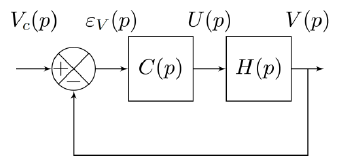
\includegraphics[width=.7\linewidth]{73_01}
\end{center}

 $H(p)=\dfrac{K_N}{(1+T_m p)(1+T_e p)}$ avec $K_N = \SI{20}{ms.^{-1}V^{-1}}$, $T_m = \SI{5}{s}$, $T_e = \SI{0,5}{s}$.
 
 \begin{obj}
\begin{itemize}
\item  Exigence 1.2 : Garantir un déplacement du chariot de vitesse : 
\begin{itemize}
\item  1.2.3 Précision :
\begin{itemize}
\item Erreur statique pour une entrée $v_c(t)=V_0 u(t)$ avec $V_0 = \SI{8}{m.s^{-1}}$ : $E_S = \SI{0}{m.s^{-1}}$.
\item Erreur de trainage pour une entrée $v_c(t)=\gamma_0 t  u(t)$ avec $\gamma_0 = \SI{1,6}{m.s^{-2}}$ : $E_T \leq   \SI{0,16}{m.s^{-1}}$.
\end{itemize}
\end{itemize}
\end{itemize}
 \end{obj}
 Le concepteur choisit un correcteur Proportionnel Intégral : $C_1(p)=\dfrac{C}{T_i p} \left(1+T_i p\right)$ avec $T_i = T_m$.
 
 
 
\question{Déterminer les expressions littérales de l'erreur statique $E_S$ (consigne : échelon d'amplitude $V_0$) et de l'erreur de trainage $E_T$ (consigne : rampe de pente $\gamma_0$) de cet asservissement corrigé avec $C_1(p)$ en fonction de la consigne, du gain $K_N$ et des paramètres du correcteur et $C$  et $T_m$.}
\ifprof
\else 
\fi

\question{ En déduire la condition (notée $C_{\varepsilon}$) sur le gain $C$ du correcteur permettant de satisfaire l’exigence 1.2.3 du cahier des charges.}
\ifprof
\else 
\fi

On choisit finalement un correcteur PID : $C_2(p)=C\left(1+\dfrac{1}{T_i p}+T_d p \right)$ avec $T_i = 2 T_e$ et $T_d = \dfrac{T_e}{2}$.

\question{Montrer qu'on peut mettre ce correcteur sous la forme  $C_2(p)= \dfrac{K}{p}\left(1+Tp\right)^2$ et donner les expressions de $K$  et de $T$ en fonction de $C$ et $T_e$.}
\ifprof
\else 
\fi


\question{Donner l'expression de la fonction de transfert en boucle ouverte du système corrigé.}
\ifprof
\else 
\fi

\question{Déterminer les expressions littérales de l'erreur statique $E_S$ (consigne : échelon d'amplitude $V_0$) et de l'erreur de trainage $E_T$ (consigne : rampe de pente $\gamma_0$) de cet asservissement corrigé.}
\ifprof
\else 
\f

\question{ En déduire la condition sur la valeur du gain $K$ du correcteur permettant de satisfaire l’exigence 1.2.3 du cahier des charges.}
\ifprof
\else 
\fi

\ifprof
\else

\noindent\footnotesize
% \fbox{\parbox{.9\linewidth}{
% Éléments de corrigé : 
% \begin{enumerate}
  % \item $\varepsilon_{\text{con \%}} = \dfrac{1}{1+K_PK_m K_{\text{pom}} K_{\text{cap}} }$;
  % \item $K_P > 19$;
  % \item $\varepsilon_{\text{pert}} = \Delta Q_e \dfrac{K_f}{1+K_{\text{cap}}K_PK_mK_{\text{pom}}}$;
  % \item $K_P > 2,19$.
  % \item $K_P < 0,125$. Il est impossible de vérifier les trois conditions avec un correcteur proportionnel.
% \end{enumerate}}}
\normalsize

\begin{flushright}
\footnotesize{Corrigé  voir \ref{C2:03:prec:73}.}
\end{flushright}%
\fi